 \documentclass[10pt]{article}
\usepackage[utf8]{inputenc}
\usepackage{natbib}
\usepackage{graphicx}
\usepackage[margin=0.75in]{geometry}
\usepackage{url}
\usepackage{amsmath}
\usepackage{comment}
\usepackage[utf8]{inputenc}
\usepackage[T1]{fontenc}
%\usepackage[font={small,it}]{caption}
%\usepackage[font={it}]{caption}
%\usepackage{fancyhdr}
%\pagestyle{fancy}
%\fancyhf{}
%\lfoot{Iain Mclaughlan}
%\rfoot{s1524154}

\usepackage{listings}
\usepackage{color}
 
\definecolor{codegreen}{rgb}{0,0.6,0}
\definecolor{codegray}{rgb}{0.5,0.5,0.5}
\definecolor{codepurple}{rgb}{0.58,0,0.82}
\definecolor{backcolour}{rgb}{0.95,0.95,0.92}

\title{Precision Refrigerator}
\author{Iain McLaughlan\\ s1524154 }
\date{\today}

\begin{document}

\maketitle
\begin{abstract}
A precision refrigerator was built and controlled using a raspberry pi to precisely control the temperature of wine (water) by toggling the on/off state of a Peltier\cite{peltier} cooling unit. The efficiency of this cooling unit was then tested by comparing the energy consumed to change the temperature of the water with the specific heat capacity of water. The fridge was found to have a percentage efficiency of ............ \%. Following this different methods for determining the on/off state of the Peltier were used. These converge on an aim temperature with different rates and efficiency's. A scoring system was devised to compare different convergence methods and the advantages and disadvantages of each were compared.
\end{abstract}

\section*{Introduction}
Micro controllers can be used for a wide range of different applications. These applications in embedded systems and can range from driving robots\cite{robomicro} to burglar detection \cite{microburg}. A micro controller refers to a small computer that is usually based on a single integrated circuit. This single circuit often contains a CPU, some form of memory and usually some form of input/output (I/O) peripherals. In recent times micro controllers and in turn micro processors have became significantly more powerful and can control much more complex systems as a result of this.\\

One application of a micro controller is in the function of a precision refrigerator. Here a micro controller can use various inputs to control the temperature of various objects. Knowing and being able to control the temperature of objects with a high level of precision is vary important in different fields. For example during experiments looking at reactions at phase boundaries\cite{microfluidic} being able to precisely control the temperature to keep the substance at a desired level is very important to obtain reliable results.\\

To precisely control the temperature of a substance it is useful to understand where and how much energy is required to heat and cool it. The energy required to change the temperature of a substance is determined by the heat capacity. The heat capacity ($C$) of a substance is defined as the ratio of heat transferred ($Q$) to or from the system and the resulting change in temperature ($T$) of the substance.  % The heat capacity is measured in $kJ/kg K$.

\begin{equation}\label{eq:heat_cap}
    C(T) = \frac{\delta Q}{dt}
\end{equation}

The heat capacity changes depending on the substance that is being heated. On top of this the heat capacity also varies with temperature and what variables are free to change and which are constrained i.e. constant pressure temperature changes vs constant volume temperature changes.\\

\begin{figure}[h!]
    \centering
    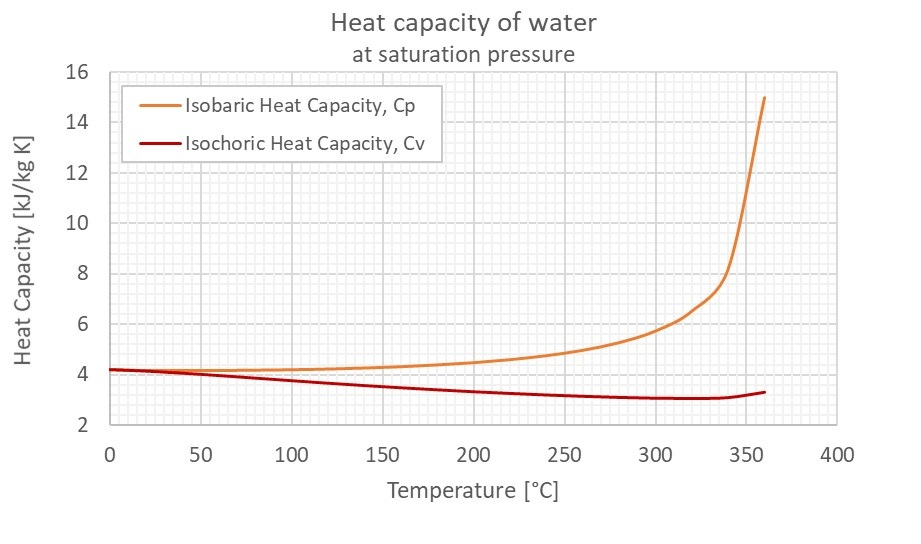
\includegraphics[scale=.75]{Heat_capacity_C.jpg}
    \caption{\it{The heat capacity of water varying differently when kept at constant pressure compared to being kept at constant volume\cite{heat_cap}.}}
    \label{fig:heat_cap_water}
\end{figure}

This variation can be seen in Figure \ref{fig:heat_cap_water} where the heat capacity of water varies differently depending on which state variable is kept constant (either pressure of volume). \footnote{At temperatures close to $0^oC$ the difference in heat capacities Cp and Cv are approximately equal and only noticeably start to diverge from one another at temperatures close to $50^oC$.}\\

Now knowing the energy required to change the temperature of the substance, being able to measure the amount of energy being transferred to the substance is important (i.e. the efficiency). The efficiency of something is defined as the ratio of the useful work produced to the total energy expended. In the case of a refrigerator this is the ratio of the energy supplied to the cooling unit compared to the energy actually used to cool.\\

\begin{figure}[h!]
    \centering
    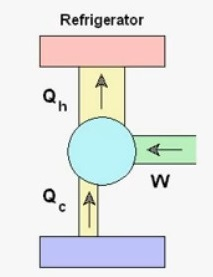
\includegraphics[scale=.75]{ref.jpg}
    \caption{\it{Energy movement through a refrigerator, transferring heat from a cold source, Qc, to a hot source, Qh, by providing work energy, W \cite{fridge}.}}
    \label{fig:fridge}
\end{figure}

Refrigerators operate by supplying work to move heat from a cold source to a hot source. The flow of heat for this process can be seen in Figure \ref{fig:fridge}. The efficiency ($\eta$) of the refrigeration process is given by;
\begin{equation}
    \eta = \frac{Q_C}{Q_H-Q_C}=\frac{Q_C}{Q_H/Q_C - 1}
\end{equation}

In the ideal circumstance where all of the work available is used to move heat is given by the Carnot efficiency\cite{carnot}. In this idealised case the efficiency is purely determined by the temperature ($T$) of the heat reservoirs.
\begin{equation}
        \eta_c = \frac{T_C}{T_H-T_C}=\frac{T_C}{T_H/T_C - 1}
\end{equation}
This is an idealised case describing the maximum efficiency, in reality it is impossible to reach this efficiency. 


% RPI Not a micro processor or micro controller but system on chip


\section*{Aims}
\begin{itemize}
    \item Build a circuit that measures the temperature of a substance and can control the on/off state of a Peltier heat pump\cite{peltier} to control the cooling of the substance. 
    \item Measure the cooling efficiency of the cooling circuit when cooling a known volume of water by a known amount.
    \item Construct several convergence methods which determine the on/off state of the Peltier depending on given inputs and compare their abilities at precisely controlling the temperature of the water.
\end{itemize}
\section*{Method}
The Peltier heat pump cooling chip was controlled using a breadboard circuit was built using a Raspberry Pi\cite{rpi} as a system on a chip micro controller. The chip was powered using an external power supply which was connected and disconnected using a transistor. A python script was written to control the state of the transistor depending on temperature readings from a thermometer. \\

\subsection*{Thermometer Calibration}

The circuit was initially set up with a Programmable Resolution 1-Wire Digital Thermometer (DS18B20) thermometer\cite{thermometer}. This thermometer has a programmable precision of 9 to 12 bits. In 12 bit mode this gives the thermometer a highest precision where it is able to read at $2^{-4o} C (0.0625^o C)$. This was tested with a short python script which reads the temperature of the thermometer every 2 seconds\ref{app:therm_test}. A second thermometer was connected in parallel with the first and was tested in the same way. Over a period of 60 seconds with the thermometer probes measuring the room air temperature near to one another, the temperature from both thermometers were recorded. The temperatures were found to be consistent with one another with only small fluctuations which averaged out at the same value for both instruments. Since both probes measured the same temperature there was no systematic offset needed to be built in to further measurements. If a systematic error was found then an average of the two probes would have been found and the difference between the mean of one probe and the mean of both would be added to all further readings.\\

\subsection*{Peltier Setup}
The Peltier was connected to a ********* power supply. This was in turn connected to a ******* transistor which acted as a switch and could be controlled by a Raspberry Pi by toggling the state of one of its GPIO (general purpose input output) pins between a high and a low voltage. When the input voltage to the transistor was high the transistor switched on which completed the Peltier circuit activating the cooling chip using the ******* power supply. When the voltage was low the transistor switched off which disconnected the Peltier circuit and stopped the cooling chip from receiving power.\\

The cooling chip circuit was tested by toggling on and off the transistor with the power supply set to a low voltage and current. The chip was held to check that one side heated as the other side cooled when powered. This was only done in short bursts as leaving the chip running for long periods of time when not connected to a heat sink can damaged the chip. \\

Once the Peltier and thermometer were working and tested the Peltier chip was placed on a heat sink. On top of this was placed a small beaker filler with $50ml$ of water and the thermometer probe was placed in the water to measure the temperature of the water. A second thermometer was set up to read the ambient room temperature near the water beaker.


**** Set up diagram? ****

\subsection*{Controlling the Cooling Chip}
Several methods were made which determined the state of the cooling chip which aimed to converge the temperature of the water down to a target temperature. In all methods a precision range was set which corresponded to the precision with which the thermometer could measure (in some cases this was increased to see different responses). This was done to allow for inaccuracies in the temperature readings; prevent the cooling chip from rapidly switching on and off which could damage it; and provide an acceptable range around the aim temperature which would be counted as the same as the aim temperature (aim temperature $\pm$ precision = aim temperature).\\

These methods worked using the following rules:\\ % converge(), hysteretic_conv(), rate_limit_conv(), pre_empt_conv()

1 (Converge). If the temperature of the water was above the aim temperature plus the precision then the chip was switched on. If the temperature of the water was below the aim temperature minus the precision then the chip was turned off.\\

2 (Hysteretic$\_$conv). This method works by realising that since the ambient temperature is taken to be greater than the cooled temperature then the heating of the water will happen faster than the cooling process. To combat this the cooling chip was activated when the temperature was below the aim temperature minus half of the precision. This reduces the relative heating phase.\\

3 (Rate$\_$limit$\_$conv). \\

4 (Pre$\_$empt$\_$conv). Here the rate of temperature change is used to try and pre-empt the point at which the temperature will become greater than or less than the aim temperature and toggle the state of the cooling chip accordingly. This is done using the idea that the temperature of the water will continue to change even after the state of the chip has been changed. For example, when the water is heating, if the rate ($degrees/s$) added to the current temperature will be greater than the aim temperature then the cooling chip will be turned on to start the cooling process before the temperature has fully risen to the aim temperature. This rate can be multiplied by an estimated change factor i.e number of seconds for an effect to be realised, to try and work closer to the aim temperature.\\

To compare the different convergence methods a scoring system was devised which looks at temperature measurements over a test period and finds the fraction of these which were within the precision range of the desired temperature. The test range was chosen to only start when the temperature had reached the aim temperature so as to only count the region around an aim temperature and not while cooling. \\

In addition to this the efficiency of the cooling system was measured. This measurement was made during the initial cooling phase before the aim temperature had been reached for the first time. This was done my recording the time ($t$) between when the chip was first turned on and when the aim temperature had been reached. This time was multiplied by the power provided from the power source ($P=IV$) to give a total energy used to cool. This was then compared to the energy required to cool the water by the same temperature difference ($\Delta T$) using the known specific heat capacity ($c$) and mass ($m$) of the water. The ratios of these energies was used to find the efficiency of the overall cooling system:
\begin{equation}
    \eta_{sys} = \frac{EnergyToCoolWater}{TotalEnergySupplied} = \frac{cm\Delta T}{Pt}
\end{equation}


% using the heat capacity of water at room tmp
\section*{Results and Discussion}

\subsection*{Discussion}
Therm calibration could be improved by measuring consistency over a range of temperatures.
Heat dispersion throughout the water.
Heating issues with heat sinks n that
\section*{Areas of Further Research}


\section*{Conclusion}

\bibliographystyle{unsrt}
\bibliography{references}



\newpage
\appendix


\newpage
\section{Python Data Analysis Code}\label{ap:code}

\lstdefinestyle{mystyle}{
    backgroundcolor=\color{backcolour},   
    commentstyle=\color{codegreen},
    keywordstyle=\color{magenta},
    numberstyle=\tiny\color{codegray},
    stringstyle=\color{codepurple},
    basicstyle=\footnotesize,
    breakatwhitespace=false,         
    breaklines=true,                 
    captionpos=b,                    
    keepspaces=true,                 
    numbers=left,                    
    numbersep=5pt,                  
    showspaces=false,                
    showstringspaces=false,
    showtabs=false,                  
    tabsize=2
}
 
\lstset{style=mystyle}
 
% \begin{document}
% \lstinputlisting[language=python]{}
% \end{document}

\end{document}